\documentclass[letterpaper]{article}
\usepackage{underscore}
\usepackage[left=2.0cm, right=2.0cm, top=2.0cm]{geometry}
\usepackage[utf8]{inputenc}
\usepackage{graphicx}
\usepackage{graphics}
\usepackage[spanish]{babel}
\usepackage{lipsum}
\usepackage{float}
\usepackage{subfigure}
\usepackage{color}

\title{EV\_2\_7\_diseño\_de\_un\_modulador\_de\_pulso\_(PWM\_con\_amp\_op\_y\_transistores)}
\author{Ledesma Hernández Miguel Ángel}
\date{22/10/2019}

\begin{document}
\maketitle
\vspace{8cm}
\begin{center}
\begin{large}
4-A Mecatrónica
Universidad Politécnica de la Zona Metropolitana de Guadalajara
\end{large}
\end{center}
\newpage
\begin{large}
El PWM por sus siglas en inglés Pulse with modulation/pulso con modulación es una forma facil de controlar señales dígitales que nos puede llegar a servir para variar la energía que se le envia a una carga o para codificar información dentro de esta señal.\\
Esta es un tipo de señal muy simple. Como ejemplo de una señal digital es cuando tenemos un botón que permite el flujo de la corriente por el circuito, solo con presionarlo. al tocarlo podremos ver en un osiloscopio la siguiente forma:
\begin{figure}[hbtp]
\centering
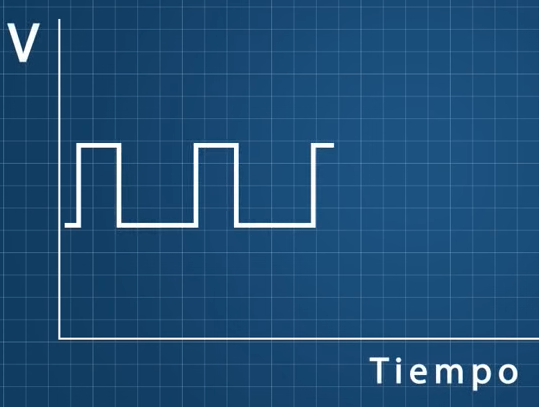
\includegraphics[scale=.4]{bianriografica.png}
\caption{Voltaje con respecto a tiempo en botón}
\end{figure}

una forma cuadrada por que el voltaje aumenta inmediatamente de no tener nada, 0V a tener algo que seria estado boleano 1 es decir un voltaje como puede ser 5V o cualquier cantidad, la señal solo muestra datos binarios, por tanto solo se encontrará 1's y 0's como se ve en la imagen anterior, tambien lo podemos representar como bajo y alto.\\
cuando la señal alcanza al maximo voltaje podemos decir que está en estado alto(1) y cuando no hay ningun voltaje por esa señal decimos que está en estado bajo(0), eso es en el caso de digitales. Pero también se puede usar para controlar el giro de un motor o el brillo de una luz; Cuando es el cazo, estos pulsos se generan a altas frecuencias y al variar el tiempo de cada pulso se puede controlar el voltaje promedio en la salida.
Si tenemos un voltaje de 10V y un $\%$ del tiempo alto y el otro bajo decimos que tenemos un voltaje medio de 5 v, pero cuando tenemos un $\%$ de tiempo más bajo, es decir que las pulsaciones estén mas cerca una de otra tendremos un voltaje medio más cercano al voltaje total; esto sirve para controlar un motor, led, foco etc...\\
como dato curioso, las interferencias son tan rapidas que son casi imperceptibles para el ojo humano.\\

Para lograr estas pulsaciones tan rapidas que claramente son imposibles de alcanzar con un motro se crean circuitos eléctricos que genere pulsos a grandes velocidades y sin la necesidad de un botón.\\

Uno de esos es con un 555 que nos ayudará a regular los pulsos de carga de un capacitor y con ello modular el tiempo con respecto al voltaje a esto le llamamos ppm.\\
\end{large}
para poder crear un PWM debemos primero tomar un 555, un potenciometro de 10k, dos resistencias de 1k, un led, capacitores y una fuente de 12V
si queremos hacerlo con un foco será con un mosfet
 simplemente conectamos concorde al datasheet del 555\\
\begin{figure}[hbtp]
\caption{555 datasheet}
\centering
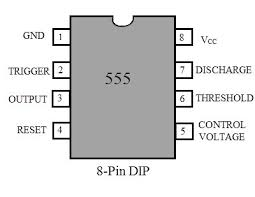
\includegraphics[scale=1]{555.jpeg}
\end{figure}

circuito
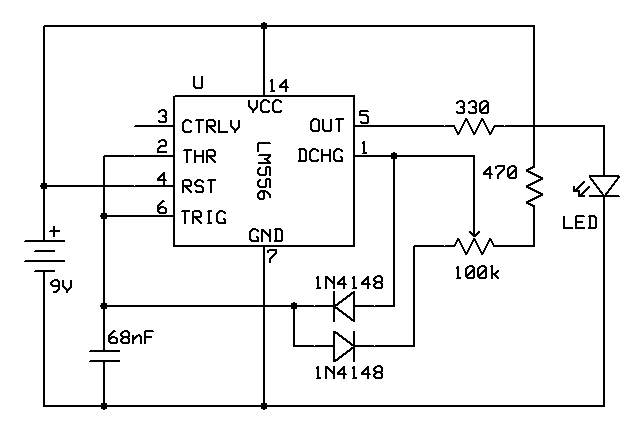
\includegraphics[scale=.5]{PWM.PNG} 
\\Para poder finalizar mostrando con un osiloscopio el ancho de puslo de banda
\newpage
Bibliografias: \\
Autor:Joyplanes RC, fecha de consulta: 21/10/19, fechas de subida: 1 feb 19 titulo del video:PWM Explicado | Cómo hacer un controlador de velocidad de motores DC, Recuperado de :https://youtu.be/Q2N2OEicXJE\\

Autor:
RincónIngenieril
, fecha de consulta: 21/10/19, fecha de subida: 19/12/17, titulo de video:Qué es PWM y para que sirve - Una explicación sencilla y detallada, Recuperado de : https://www.youtube.com/watch?v=GnlmVMHA_wQ.

\end{document}

